\section{Flow in a channel with heterogeneously charged walls}

Now a channel with walls charged with a varying charge is
considered. The walls are charged piecewise constant with every second
piece positive and negative respectively, see
fig. \ref{fig:res:h_setup}. The length of the charged sections are
chosen as $d/4$ where $d = 10 \mu$m is the width of the channel. The
flow is electroosmotic and driven by an external field of $50$ kV/m.

\begin{figure}
  \centering
  \subfloat[Heterogeneous wall charge
    ]{\label{fig:res:h_setup}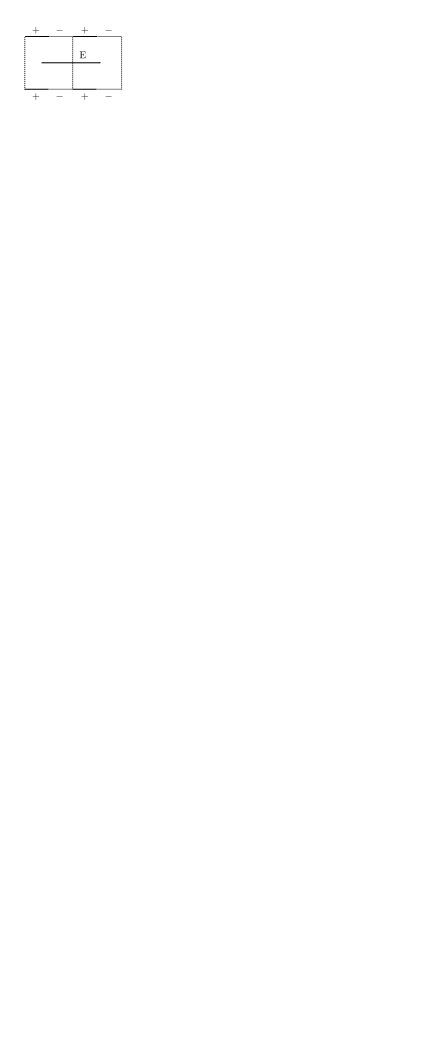
\includegraphics[width=0.35\textwidth]{fig/hetro_setup.pdf}}      
  \hspace{5pt} \subfloat[Array of charged squares
  ]{\label{fig:res:square}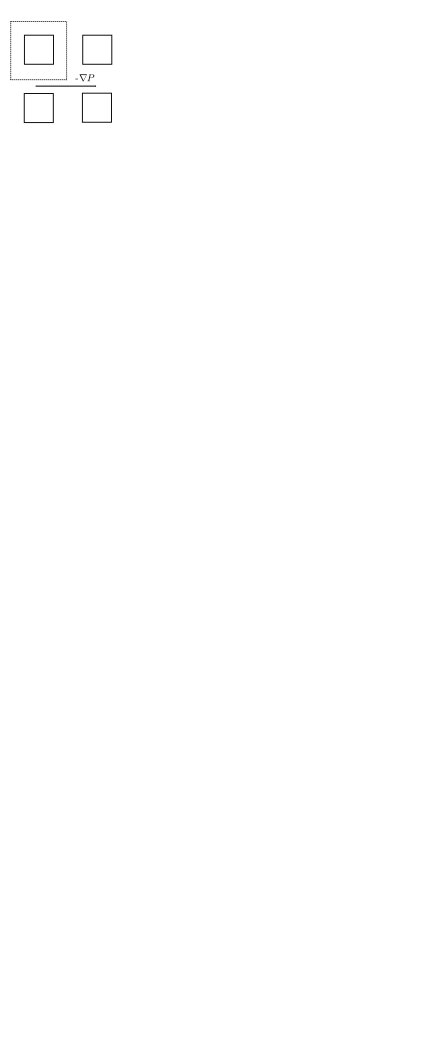
\includegraphics[width=0.35\textwidth]{fig/square_setup.pdf}}
  \caption[Sketch of setups for two physical 2D systems.]{Sketch of
    setups for the two physical 2D systems that are modelled. In (a),
    electroosmotic flow through a channel with heterogenously charged
    walls. In (b), pressure driven flow in an array of squares.}
  \label{fig:res:setup}
\end{figure}

The resulting velocity profile together with the charge distribution
of positive ions in the steady state is presented in
fig. \ref{fig:res:hetro}.

\begin{figure}
  \centering
  \subfloat[Velocity field
    ]{\label{fig:res:ta1}\includegraphics[width=0.32\textwidth]{fig/field_hetro.pdf}}      
  \hspace{5pt} \subfloat[$|\ubf|$
  ]{\label{fig:res:ts2}\includegraphics[width=0.32\textwidth]{fig/u_hetro.pdf}}  
\hspace{5pt} \subfloat[$\C_+$
  ]{\label{fig:res:t2}\includegraphics[width=0.32\textwidth]{fig/c_hetro.pdf}}
  \caption[Velocity field for flow in channel with heterogeneously
    charged walls.]{Visualised velocity field (a), magnitude of the
    velocities (b) and charge concentration of positive ions for a
    flow in a 2D channel with heterogeneously charged walls. A
    constant electric field of 50 kV/m drives the flow. The velocity
    field in (b) varies from $0.02 \mu$m/s (blue) to $2.2 \mu$m/s
    (red). The charge concentration in (c) varies from $0.45\C_0 $
    (blue) to $2.12\C_0$ (red).}
  \label{fig:res:hetro}
\end{figure}

There is an accumulation of positive and negative ions in the vicinity
of the negative and positive charged boundaries respectively. In the
middle of the channel, the fluid is neutral.

The vortexes obtained agrees qualitatively with those computed in
\cite{lbm-wang}. This kind of system is for example used in mixing of
charge fluids \cite{mixing}. Varying charges are imposed on the
boundary of a domain and an electric field is applied, this results
typically in a flow similar to the vortexes obtained here.

